\documentclass[../report.tex]{subfiles}

\begin{document}
\graphicspath{{img/}{../img/}}


\section{Gantt planl�gning}
Gantt er en udbyggelse af den klassiske tidsplan. Den er lavet for at give et bedre overblik over de forskellige planlagte opgaver i forhold til hinanden. Hvor en klassisk tidsplan i form af en tabel er fokuseret p� tidsperioderne, er et Gantt diagram fokuseret p� arbejdsopgaverne.\\

Figur~\ref{fig:Gantt} viser Gantt diagrammet for target projektet. Aktiviteterne p� diagrammet er meget abstrakte, og det kommer af target-projektgruppens valg af procesmodel. De har valgt at bruge Scrum til software udviklings aktiviteterne, hvilket de i Gantt diagrammet regner med udg�r cirka halvdelen af arbejdstiden. Da Scrum er en iterativ proces bliver aktiviteterne nedbrudt og valgt l�bende, og de har alts� valgt ikke bare at holde disse aktiviteter abstrakte i Gantt diagrammet, men ogs� aktiviteter f�r og efter det relle Scrum forl�b. Scrum forl�bet bliver beskrevet mere i afsnit \ref{sec:Scrum}.\\




\begin{figure}[H]
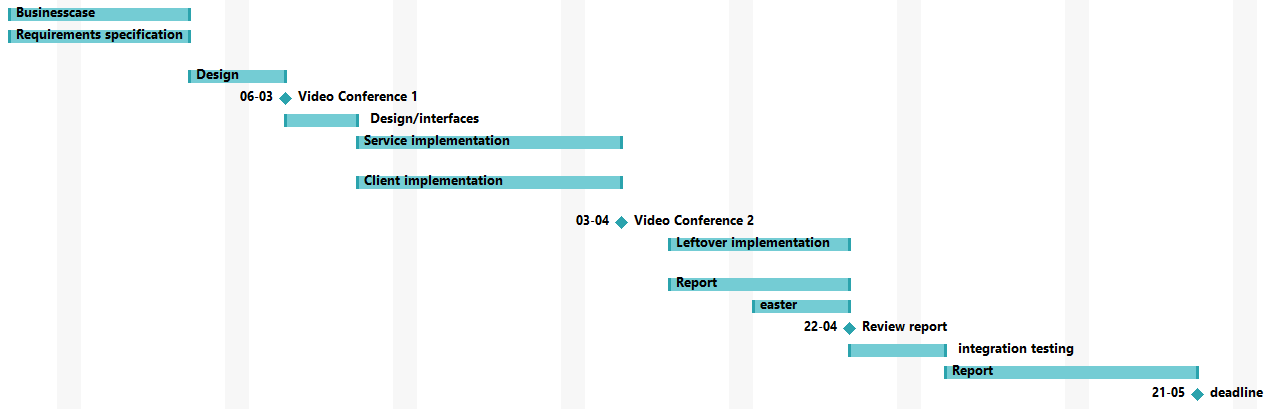
\includegraphics[scale=0.45]{TargetProjectGantt.png}
\caption{Gantt diagram for target projektet}
\label{fig:Gantt}
\end{figure} 

Gantt diagrammet vinder stort inden for overblik mod den klassiske tidsplan, men i n�ste kapitel kigges der p� et andet alternativ til aktivitetsplanl�gning.



\end{document}